\documentclass[12pt]{article}
\usepackage[T1]{fontenc}
\usepackage[slovak]{babel}
\usepackage{mathptmx}

\usepackage{caption}
\usepackage{subcaption}
\usepackage{indentfirst}

\usepackage[numbers]{natbib}
\bibliographystyle{rusnat}

\usepackage[width=\textwidth]{svg}

\usepackage[a4paper,left=35mm,
                    right=25mm,
                    top=25mm,
                    bottom=25mm]{geometry}

\linespread{1.5}   % 1.5 riadkovanie

\AddToHook{cmd/section/before}{\clearpage}

\def\nazovprace{Botanica - simulátor rastlín na báze celulárnych automatov}
\def\autori{František Knapec, Michael Sklenka, Marek Beňo}

\begin{document}

\begin{titlepage}
	\setlength{\parindent}{0pt}

	\begin{center}
		Gymnázium \\
		Veľká okružná 22, 010 01 Žilina

		\vspace{7cm}
		\Huge \nazovprace

		\vspace{1.13cm}
		\Large Stredoškolská odborná činnosť

		\vspace{2.12cm}
		\normalsize Č. odboru: 11
	\end{center}

	\vfill

	\begin{minipage}{0.75\textwidth}
		Riešitelia: \autori \par
		Ročník štúdia: 4.
	\end{minipage}
	\hfill
	\begin{minipage}{0.23\textwidth}
		\hfil % basically align right
		\begin{tabular}{rc}
			Mesto: & Žilina \\
			Rok:   & 2025
		\end{tabular}
	\end{minipage}
\end{titlepage}

\begin{titlepage}
	\setlength{\parindent}{0pt}

	\begin{center}
		Gymnázium \\
		Veľká okružná 22, 010 01 Žilina

		\vspace{7cm}
		\Huge \nazovprace

		\vspace{1.13cm}
		\Large Stredoškolská odborná činnosť

		\vspace{2.12cm}
		\normalsize Č. odboru: 11
	\end{center}

	\vfill

	\begin{minipage}{0.75\textwidth}
		Riešitelia: \autori \par
		Ročník štúdia: 4. \par
		Školiteľ: Ing. Tomáš Milet, PhD.\par

	\end{minipage}
	\hfill
	\begin{minipage}{0.23\textwidth}
		\hfil % basically align right
		\begin{tabular}{rc}
			\\ \\
			Mesto: & Žilina \\
			Rok:   & 2025
		\end{tabular}
	\end{minipage}
\end{titlepage}

% zapocitaj strany
\setcounter{page}{3}


\thispagestyle{empty}

\null
\vfill

\noindent
\textbf{Čestné vyhlásenie:}

Prehlasujeme, že sme prácu na tému
\nazovprace \space
vypracovali samostatne s~použitím literatúry uvedenej v~zozname použitej literatúry.
Zároveň prehlasujeme, že sme predloženú písomnú prácu neprihlásili a ani neprezentovali
v žiadnej inej súťaži, ktorá je pod gestorstvom MŠMVVaŠ SR. Sme si vedomí zákonných dôsledkov,
ak v~nej uvedené údaje nie sú pravdivé.

\vspace{4cm}

\newpage


%
% Poďakovanie (nepovinné)
%

% \thispagestyle{empty}
% 
% \null
% \vfill
% 
% \noindent
% \textbf{Poďakovanie}
% 
% \noindent
% Toto je poďakovanie
% 
% \vspace{8cm}
% \newpage


\thispagestyle{empty}
\tableofcontents

%
% The work :)
%

\section*{Úvod}
\addcontentsline{toc}{section}{Úvod}

Väčšina hier s~otvoreným procedurálne generovaným svetom vníma rastliny iba ako
jednoduché assety pre skrášlenie sveta. Pre veľa hier je tento prístup ideálny,
avšak ním prichádzajú o pestrosť a zaujímavosť, ktorú ponúkajú simulácie.
Simulovanými rastlinami môžu benefitovať hlavne survival hry (hráč sa snaží
prežiť, zväčša v nepriateľskom prostredí) a sandbox hry (svet je upravovateľný
hráčom).

Mimo vizuálne pekného prostredia ponúkajú simulované rastliny aj možnosti
mnohých unikátnych mechaník ako napríklad možnosť geneticky
modifikovať rastliny, čím by hráč mohol napríklad zvýšiť produkciu svojej záhrady
v survival hrách.

Táto práca sa zaoberá aplikáciou demonštrujúcou jednoduchý algoritmus
pridávajúci rastlinám možnosť reagovať na okolité prostredie. Aplikácia
simuluje a vykresľuje rastliny v procedurálne generovanej časti sveta.
Rastliny reagujú na množstvo látok (dusík, draslík a fosfor) v zemine,
množstva vody a svetla pomocou ich genómu.

Najprv sú vysvetlené základné pojmy, algoritmy a praktiky používané pri tvorení
herného sveta. Následne je predstavená aplikácia, ktorá demonštruje algoritmus
pre jednoduché spestrenie rastlín vo svete. Záver práce sa venuje možným
zlepšeniam aplikácie a ďalším využitiam simulovania rastlín v hrách
s otvoreným svetom.


\section{Problematika a prehľad literatúry}

Táto práca sa zaoberá implementovaním rastlín do digitálnej podoby a následným
simulovaním ich správania relatívne k podmienkam, v ktorých sa nachádzajú,
ako aj k iným rastlinám v ich okolí. Jej súčasťou je aj vyobrazenie
rastlín v trojrozmernom priestore. Pôjde aj o schopnosť dlhodobého
pozorovania ekosystému naprieč časom.

Ľudia k problému tvorenia digitálnych rastlín pristupovali rôznymi spôsobmi,
avšak väčšina z nich len realistické rastliny vykresľovala, pozri napríklad
známy príklad L-systémov, \cite{wiki:L-system}
ktorý je založený na opisovaní štruktúry rastlín
sériou pravidiel, ako je napr. otočenie, vytvorenie úsečky alebo
vrátenie sa na určitú pozíciu. Ďalej sa štruktúra zdokonaľuje za pomoci
algoritmu, ktorý nahrádza časti jej série pravidiel za iné, dopredu určené
a detailnejšie série. Tento postup dokáže vytvoriť celkom realistické rastliny
ako je znázornené na obr. \ref{obr:priklad l-systemu}.

\begin{figure}[ht]
	\centering
	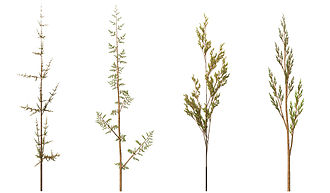
\includegraphics[width=0.5\textwidth]{res/Fractal_weeds.png}
	\caption{Príklad tráv vygenerovaných s použitím L-systému v 3D}

	\footnotesize (zdroj: https://en.wikipedia.org/wiki/L-system)

	\label{obr:priklad l-systemu}
\end{figure}

Toto riešenie a jemu podobné však dané rastliny len vytvárajú, no našim cieľom
je aj simulovať ich život.


\subsection{Spôsoby simulovania rastlín}

Kvôli samotnej simulácii vzniklo viacero metód simulovania s vlastnými kladmi,
ale aj zápormi. Medzi takéto metódy patria:

% TODO: ukážky, citácie, zdroje
\begin{itemize}
	\item \textbf{Fyzikálne založené modelovanie} využívajúce body prepojené
	      pružnými štruktúrami, na ktoré pôsobia rôzne sily. Aj keď realistické,
	      modelovanie neumožňuje rastliny tvoriť, iba simulovať.
	\item \textbf{Simulácia pomocou strojového učenia} \cite{wiki:Machine_learning}
	      využíva štatistické
	      algoritmy, pomocou ktorých sa počítač dokáže počas tréningu učiť vzťahy medzi
	      vstupmi a výstupmi.
	\item \textbf{Celulárne automaty} \cite{wiki:Cellular_automaton}
	      je názov pre matematický model a nástroj pre simuláciu. Jedná sa
	      o starší koncept, ktorý obsahuje štvorcovú sieť so „zafarbenými“
	      políčkami. Každá farba je určitý stav, ktorý má špecifické správanie
	      závisiace od okolitých políčok.
\end{itemize}

Fyzikálne založené modelovanie, aj keď mocné, vyžaduje, aby rastliny boli
vygenerované dopredu, pred začatím simulácie a po jej spustení nie sú tieto
rastliny schopné sa ďalej vyvíjať. Navyše spôsob vyžaduje fyzikálne založenú
simuláciu, ktorá je príliš komplikovaná pre túto prácu.

Na druhej strane, strojové učenie sa stáva čím ďalej tým využívanejšie pre
riešenie všetkých možných problémov. Avšak tento spôsob je náročný na čas
a výpočtovú techniku.

A napokon celulárne automaty ponúkajú jednoduchosť a možnosť ich jednoducho
modifikovať, čo otvára pole rôznorodých využití. Vďaka týmto výhodám je simulácia
v našej práci založená na princípe celulárnych automatoch.

\subsection{Celulárne automaty}

CA sa skladá z týchto základných častí: mriežka (často štvorcová sieť)
a bunky tejto mriežky, ktoré majú vlastný stav, pričom každý stav obsahuje
určité pravidlá, ktoré zapríčiňujú správanie buniek, a tým celého systému.
Tieto pravidlá sa aplikujú každú generáciu, každé simulačné kolo.
Vďaka týmto vlastnostiam sú CA systém, ktorý je jednoduché prispôsobiť ktorýmkoľvek
požiadavkám.

Klasickým príkladom takéhoto systému je Conwayova hra života. \cite{wiki:Conway's_Game_of_Life}
V tejto hre nadobúda každá bunka štvorcovej siete jednu z dvoch hodnôt:
Buď je bunka živá alebo mŕtva. Conwayova hra života má nasledovné pravidlá:

\begin{enumerate}
	\item Každá živá bunka s menej ako dvoma živými susedmi umrie.
	\item Každá živá bunka s dvomi alebo tromi živými susedmi prežije.
	\item Každá živá bunka s viac ako tromi živými susedmi umrie.
	\item Každá mŕtva bunka s presne tromi živými susedmi ožije.
\end{enumerate}

V hre života sa nachádza veľa stabilných konfigurácií (glidery, továrne,
oscilátory, atď.) ako je vidno na obr. \ref{obr:conwayova hra zivota}.
Vďaka týmto štruktúram je Conwayova hra života Turingovo kompletná (môže
simulovať hocijaký počítač, čiže aj sama seba\footnote
{Life in life - https://www.youtube.com/watch?v=xP5-iIeKXE8}).

\begin{figure}[ht]
	\centering
	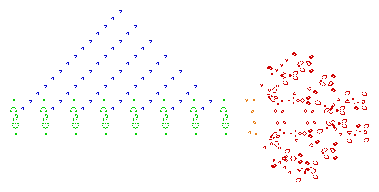
\includegraphics[width=0.9\textwidth]{res/Conways_game_of_life_breeder.png}
	\caption{Na obrázku je znázornená pohyblivá štruktúra (červená), ktorá
		za sebou zanecháva továrne (zelená) produkujúce glidery (modrá),
		jednoduché pohybujúce sa štruktúry.}
	\label{obr:conwayova hra zivota}
\end{figure}

\subsubsection{Príklady CA zamerané na simuláciu rastlín}

„Simulation of root forms using cellular automata model“ - zameriava sa na
korene rastlín a dopad premenných ako napr. živiny v pôde, voda a prekážky
v raste. Jedná sa o prácu, ktorá je viac zameraná na matematický rast koreňov,
avšak my sme rast koreňov simulovali genetikou.
% Trošku to rozveďte. Pri návrhu vlastného systému generovania rastlín sme
% sa inšpirovali rôznymi jestvujúcimi softvérovými riešeniami. Na korene
% rastlín a dopad rôznych faktorov sa zameriava...

„A Model Based on Cellular Automata for the Simulation of the Dynamics of
Plant Populations“ - zameriava sa na 2D simuláciu heterogénnej populácie
rastlín, zameraná na konkurenciu medzi druhmi, rýchlosť rastu a interakcie
s prostredím.

\section{Ciele práce}

Cieľom tejto práce je vytvorenie aplikácie schopnej tvorenia a simulácie
pseudo-rea\-listických rastlín v trojrozmernej mriežke pomocou celulárnych
automatov a implementovanej genetiky.
Tieto rastliny by mali byť schopné reagovať na prostredie v reálnom čase
a adaptovať svoje správanie, tvar a iné charakteristiky v závislosti
od podmienok, v ktorých sa nachádzajú.

Výsledkom tejto práce je softvér, Botanica, ktorý umožňuje pozorovanie
správania a vývinu simulovaných rastlín vďaka schopnostiam:

\begin{enumerate}
	\item generovať časť 3D voxelového sveta za pomoci Perlinovho šumu,
	\item simulovať rastliny vo vytvorenom prostredí pomocou vlastného
	      algoritmu inšpirovaného celulárnymi automatmi,
	\item vykresľovať túto simuláciu za pomoci grafického API OpenGL.
\end{enumerate}

Veríme, že metódy využité v Botanice sú využiteľné ako na tvorenie dynamického
a nerepetetivného prostredia vo videohrách, tak aj na viac vedecké účely
ako pozorovanie správania rastlín vo virtuálne vytvorených podmienkach
a ich ideálne charakteristiky za daných podmienok.


\section{Aplikácia (Materiál a metodika)}

Na realizovanie algoritmu sme vyvinuli jednoduchú aplikáciu, ktorá má
všetky potrebné prostriedky na demonštráciu všetkých aspektov tohto algoritmu.
Aplikácia umožňuje vizualizáciu rastu rastlín na základe celulárnych automatov
a poskytuje možnosť meniť parametre simulácie na dosiahnutie ideálneho vzhľadu
rastlín.

\subsection{Svet} \label{subsec:svet}

Svet aplikácie pozostáva z mriežky buniek o rozmeroch 32x32x32 voxelov.
Každý voxel nadobúda určitý stav. Môže sa jednať o časti rastlín (stonka, list,
koreň alebo ovocie), ale aj o časti terénu (vzduch, voda, pôda).

\subsubsection{Perlin noise}

Terén na určenie svojej výšky, aby nebol len rovina, využíva funkciu zvanú
Perlin noise. Perlin noise je spôsob generovania plynule sa meniacich náhodných
hodnôt, ktoré sa dajú skvele využiť na generovanie realistického terénu.
Čo sa týka algoritmu na jeho generovanie (obr. \ref{obr:perlinov sum}),
v určitých miestach sa vytvoria
vektory s náhodným smerom (modrý). Z bodov (červené), ku ktorým chceme pripísať
hodnoty, sa vytvoria vektory smerujúce k týmto miestam (zelené). Z náhodného
vektoru a vektoru smerujúceho z bodu sa vytvorí skalárny súčin a tým dosiahneme
hodnotu v danom bode.

\begin{figure}[ht]
	\centering
	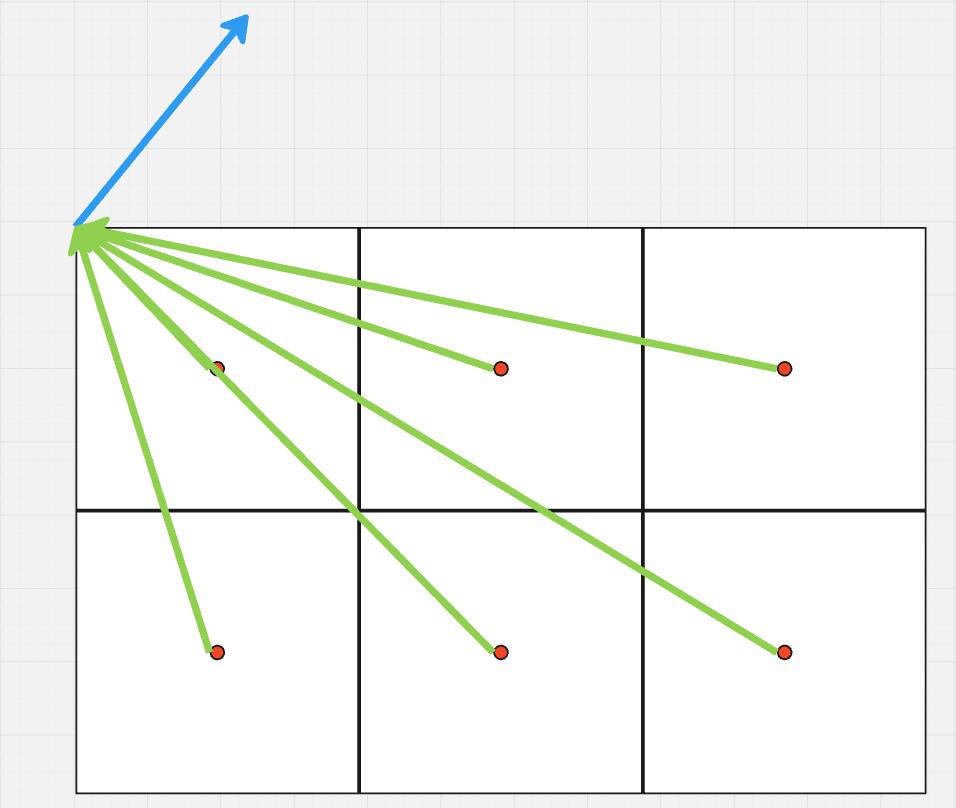
\includegraphics[width=0.5\textwidth]{res/prelinov_sum.png}
	\caption{Znázornenie generovania Perlinovho šumu za pomoci 1 náhodného
		vektoru pre 6 buniek.}
	\label{obr:perlinov sum}
\end{figure}

Avšak väčšinu času sa hodnoty nepočítajú len pre jeden náhodný vektor,
ale pre viacero (najčastejšie 4 najbližšie) a hodnoty ich skalárnych súčinov
sa spriemerujú. Často sa využíva aj viacero oktáv,\footnote{
	Oktáva je v tomto prípade mapa vytvorená Perlinovým šumom.
} pričom každá oktáva využíva
viacej náhodných vektorov, ktoré ovplyvňujú menej buniek ako predchádzajúca
oktáva. Avšak tieto oktávy vplývajú menej na výslednú hodnotu. Vyjadrenie hodnôt bodov
farebnou škálou, kde vyššie hodnoty sú viac biele a nižšie viac čierne, popisuje
obrázok \ref{obr:perlinov sum textura}.

\begin{figure}[ht]
	\centering
	
\includegraphics[width=0.4\textwidth]{res/perlinov_sum_textura.png}
	\caption{Textúra Perlinovho šumu.}
	\footnotesize (zdroj: https://en.wikipedia.org/wiki/Perlin\_noise)
	\label{obr:perlinov sum textura}
\end{figure}

Naša aplikácia vďaka jej obmedzenej veľkosti využíva 4 vektory umiestnené
na rohoch simulácie a iba 1 oktávu.

\subsubsection{Tvorenie terénu}

Tvorenie terénu sa začne vytvorením Perlinovho šumu, poďla ktorého sa určí výška terénu.
Pre každú dvojicu súradníc X a Z sa vytvorí hodnota Perlinovho šumu. Táto hodnota
bude ovplyvňovať os Y. Každý voxel, ktorého hodnota súradnice Y je nižšia alebo
rovná hodnote šumu v X, Z bude voxel terénu. Inak sa bude jednať o voxel
vzduchu. Na vytvorenie voxelov vody sa nastaví hodnota, ktorá bude označovať
hladinu vody a ak hocijaký voxel vzduchu má hodnotu Y menšiu alebo rovnú ako táto
hodnota, zmení sa na vodu. Táto hodnota nie je spojená so šumom, ide o jedno
číslo univerzálne pre celú simuláciu. Zoberme si príklad: máme zmenšenú
simuláciu a pre každú dvojicu X,Z pripadajú len 4 voxely [0,1,2,3]. Tieto voxely
majú rovnaké súradnice X, Z, ale odlišné Y, ktorá korešponduje s ich číslom.
Vytvoríme Perlinov šum, ktorý bude mať pre danú dvojicu X,Z hodnotu 1. To
znamená, že voxely s hodnotou Y 0 a 1 sa premenia na voxely pôdy a voxely 2,3
na voxely vzduchu. Ďalej hladina vody má hodnotu 2, takže voxel 2, ktorý bol
predtým vzduch, sa premení na vodu.

\begin{figure}[ht]
	\centering
	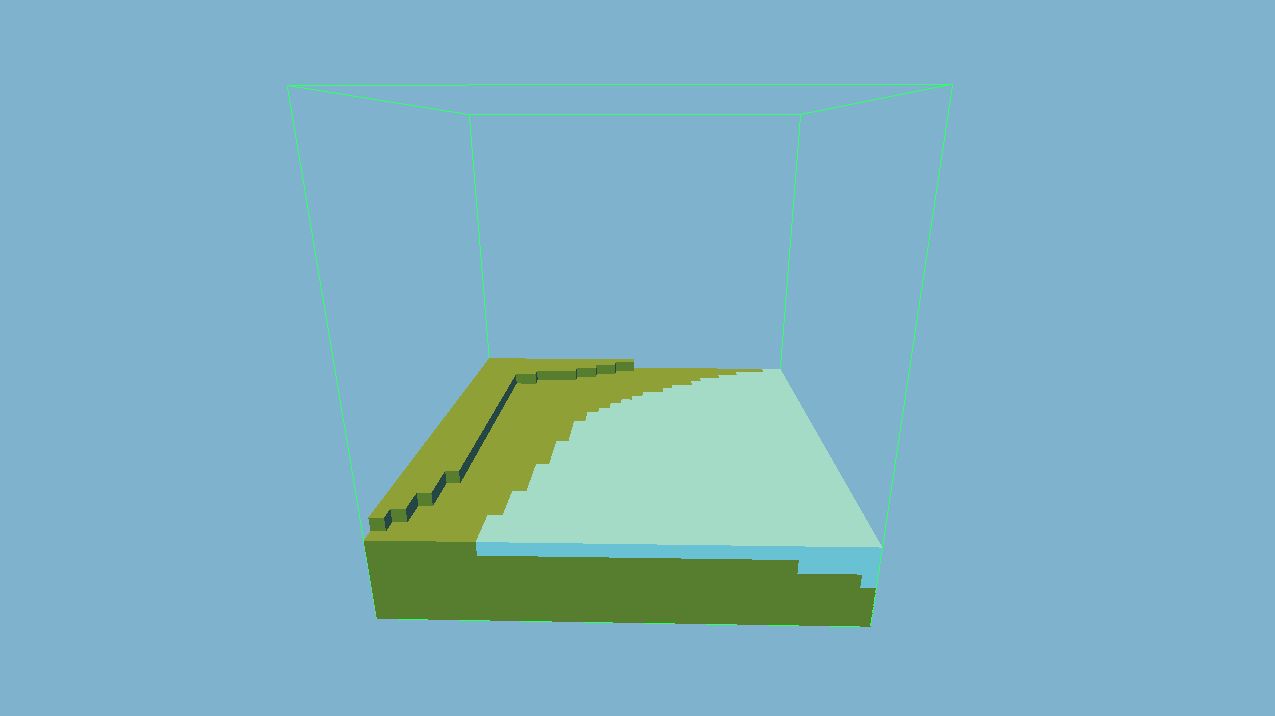
\includegraphics[width=0.9\textwidth]{res/terrain.png}
	\caption{Terén vygenerovaný touto technikou. (voda - zelená, pôda - modrá)}
\end{figure}

\subsubsection{Živiny}

Simulácia obsahuje rôzne živiny, vodu a vzduch, tieto veci rastlina potrebuje
získavať, aby rástla a prežila. Voda a vzduch majú zastúpenie v podobe ich
voxelov. Pôda obsahuje vodu a živiny. Každá živina napomáha rôznym procesom
rastliny, ako napríklad fotosyntetizovať, čerpať vodu alebo získavať viac živín.
Ich nadbytok má kladný vplyv na rastliny, avšak ich nedostatok má zase
negatívny. Toto pridáva na komplexnosti, realizme a dovoľuje nám získať rôzne
typy rastlín, podľa toho, ku ktorým živinám majú alebo nemajú prístup.
Napríklad ak rastlina nemá dostatok dusíka, ktorý je v simulátore dôležitý
na fotosyntézu, rastlina to musí kompenzovať viacerými listami, inak zanikne.
Živiny sú 3, dusík, draslík a fosfor, pričom bola snaha o to, aby napomáhali
realistickým procesom, ktoré tieto prvky vyžadujú. Draslík je nápomocný pri
absorpcii vody, takže ak má rastlina nadbytok draslíka, efektívnejšie získava
vodu. Využitie dusíka je široké, ale v simulátore je jeho funkcia obmedzená
len na zlepšenie fotosyntézy, keďže je hlavnou zložkou chlorofylu. Fosfor je
rovnako ako dusík dôležitý v rôznych častiach, avšak v simulátore je zameraný
na absorpciu živín.

\newpage
\subsection{Rastliny}

Rastliny sú v tomto simulátore objekty so spoločnou „triedou.“ Trieda je
predloha premenných a špeciálnych funkcií zvaných metód, ktoré využívajú
jednotlivé entity, taktiež známe ako objekty. Takáto šablóna nám umožňuje
jednoducho a usporiadane tvoriť rastliny, pretože nemusíme písať samostatný
kód pre každú rastlinu.

\begin{figure}[ht]
	\centering
	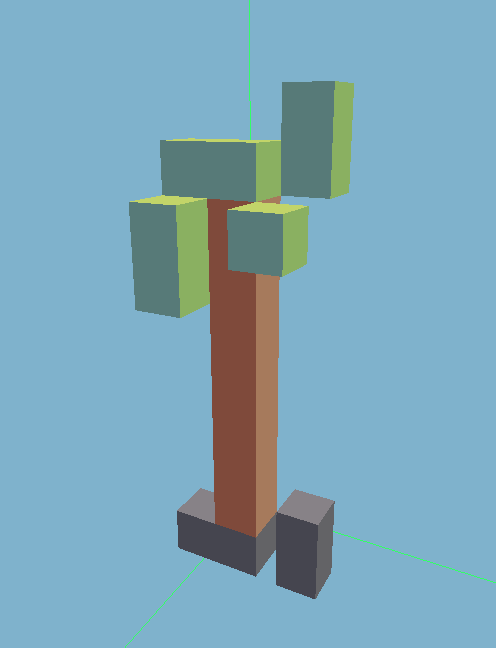
\includegraphics[width=0.5\textwidth]{res/plant.png}
	\caption{Foto rastliny z našej simulácie.}
\end{figure}

\subsubsection{Premenné v rastlinách}

Rastliny majú viacero premenných. Ich hlavnou úlohou je opísať stav rastliny.
Medzi ne patria údaje o skonzumovaných živinách za toto kolo, zoznam všetkých
voxelov, v ktorých sa nachádzajú časti rastliny a ich gény. V premenných
taktiež máme aj bonusy pre živiny. Hovoria nám o nadbytku alebo nedostatku
živín. Bonusy sú rozobrané v kapitole „Živiny“.

\subsubsection{Rastlinné voxely}

Fyzické zobrazenie rastlín sa skladá zo špecializovaných voxelov, ktoré
v mriežke reprezentujú ich časti. Tieto voxely taktiež voláme aj bunky.
Existujú 4: korene, stonky, listy a ovocie. Každá skupina buniek plní
vlastnú úlohu. Koreň má za úlohu rastline získať živiny a vodu, to dosahuje
odoberaním týchto živín z okolitých voxelov. Koreň môže vzniknúť iba na
miestach, kde je pôda. Úlohou listu je fotosyntéza, tú dosiahne tým, že
skontroluje, či políčka nad ním sú vzduch. Predpokladáme, že na voxel vzduchu
priamo svieti slnko. Stonka uskladňuje živiny pre rastlinu 
a rastie iba zvislo. Ovocie tvorí nové rastliny
s pôvodným genetickým kódom, ktorý trochu zmutuje. Na pár kôl nahrádza 1 list,
ktorý sa po premene ovocia na novú rastliny znova zmení na list.

\subsubsection{Genetika a rast}

Na základe genetiky rastliny rozhodujú, aké časti majú rásť (listy, stonka…)
a v prípade listov a koreňov existujú gény určujúce, akým smerom majú rásť.
Takže existujú 3 gény: čo má rásť, kde majú rásť korene a kde majú rásť listy.
Gén „čo má rásť“ je vo všetkých prípadoch list so 4 číslami. Sú 4, pretože sú 4
typy buniek, ktoré môže rastlina rásť: korene, listy, stonku a ovocie. Čísla
v týchto listoch označujú, ako veľmi chce daná rastlina v danej časti rásť. Takže
ak má rastlina časti označujúce stonku 2 a koreň 10, daná rastlina bude
chcieť rásť v koreni 5-krát viac ako stonka. V ktorej časti bude rastlina naozaj
rásť, sa rozhoduje náhodne. Ak sa vrátime k nášmu príkladu, dokopy $2+10=12$,
čo je prirovnateľné hodu 12-stennou kockou. Ak sa vygeneruje číslo,
ktoré je väčšie ako 2, rastie koreň, inak rastie stonka. Gény „kde majú rásť korene“
a „kde majú rásť listy“ sú rovnaké, len ako ich názov hovorí, jeden sa zaoberá
koreňmi a druhý listami. Sú to listy s 26 číslami. Je ich 26, pretože bunka má
v trojrozmernom priestore 26 susedov, ak rátame aj diagonály. Zvyšok funguje
rovnako ako gén „čo má rásť“. Takže sú tam čísla, ktoré označujú
pravdepodobnosť rastu do daného smeru. Ak sa tieto 2 gény zavolajú, vyberie
sa náhodná bunka (list alebo koreň podľa toho, ktorý gén sa zavolá), a ak
nemôže rásť do toho smeru, tak sa vyberie iná bunka, ak žiadna nemôže rásť,
vyberie sa iný smer.

\newpage
\subsection{Algoritmus}

Ako bolo spomínané, simulácia nebeží súvisle, ale v časových krokoch.
Za každý krok sa vykonajú určité akcie, tzv. cyklus. Tieto akcie slúžia na beh
simulácie a starajú sa o udalosti, ako rast rastlín, ich vznik, smrť atď.
Vďaka tomu možno algoritmus rozdeliť do nasledujúcich častí, ktoré sú spísané
chronologicky, tak ako ich simulácia vykonáva.

\begin{figure}[ht]
	\centering
	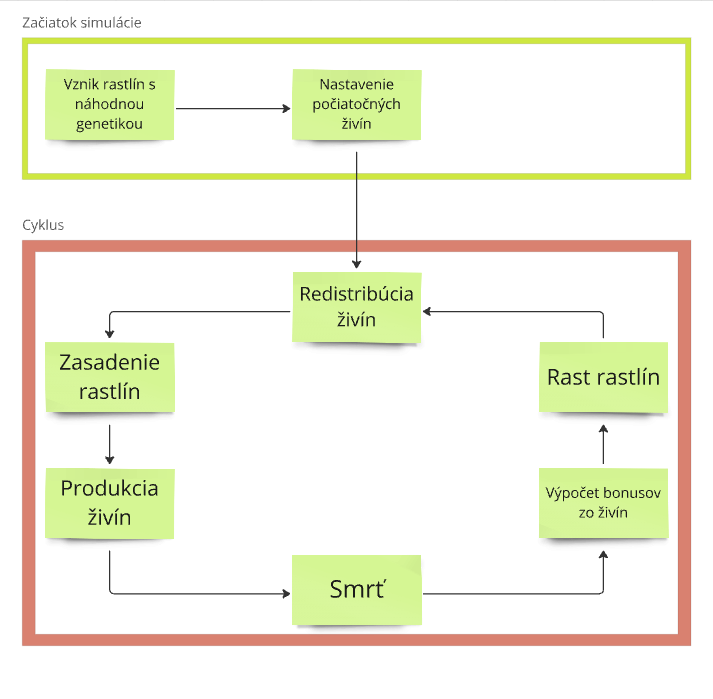
\includegraphics[width=0.7\textwidth]{res/diagram_algoritmu.png}
	\caption{Diagram algoritmu.}
\end{figure}

\subsubsection{Vznik rastlín}

Vznik rastlín je jediná časť algoritmu, ktorá nebeží v krokoch, ale iba raz, a to na začiatku
simulácie. Po vytvorení terénu sa vyberie náhodné miesto na jeho povrchu, kde
je pôda, a tam vznikne rastlina. Toto sa dá opakovať viackrát, na vytvorenie
viacerých rastlín. Takéto rastliny sa skladajú z 1 koreňa, 1 stonky a 1 listu.
Ich genetika je náhodná, keďže ju nemôžu dediť z materských rastlín, ktoré
neexistujú.

\subsubsection{Redistribúcia živín}

Redistribúcia živín je prvá akcia, ktorá sa vykonáva v každom kroku simulácie. Živiny sú totiž
ukladané v dvoch listoch, jeden permanentný, ktorý drží informácie o počte
živín a vody zo začiatku simulácie a druhý dočasný, z ktorého rastliny čerpajú.
V tomto bode je list dočasných živín obnovený na hodnoty rovné permanentnému listu.
Toto umožňuje rastlinám znovu brať živiny v novom cykle.

\subsubsection{Zasadenie rastlín}

Ak má rastlina ovocie, ktoré existuje po určitú dobu, tak sa z neho stane nová
rastlina. Rozdiel vo vzniku a zasadení je, že genetický kód nie je
vygenerovaný náhodne, ale ho rastlina zdedí zo svojej materskej rastliny,
pričom v každej časti genetiky jednu hodnotu náhodne zmení, teda „zmutuje“.

\subsubsection{Produkcia živín}

V tejto fáze rastlina získava živiny vďaka svojim bunkám, konkrétne listom
a koreňom. Listy sa pozrú na bunky horizontálne nad nimi a podľa toho, koľko
z nich je vzduch, „produkujú“ svetlo. Korene zase pozrú bunky v ich susedstve
a podľa toho generujú živiny a vodu. Koľko z okolitých buniek dokážu listy
a korene dostať, je určené samozrejme počtom živín v bunkách terénu, z ktorého
rastlina čerpá, ale rastlina nezoberie jednoducho všetky živiny v okolitom
teréne. Maximálny počet živín, ktoré dokáže bunka získať je stanovený
konštantou a jej bonusom zo živín. V stonkách sa uskladňujú živiny, čiže
rastlina nemôže skonzumovať viac ako jej to limit odvodený z počtu buniek
stoniek dovoľuje. 

Napríklad chceme fosfor. Je koreň s 5 okolitými bunkami,
pričom každá obsahuje 15 jednotiek fosforu. Konštantu produkcie máme 10,
povedzme, že máme bonus pre fosfor krát 1.2, čiže z každej dokážeme brať až 12
jednotiek. To predstavuje dokopy 60 jednotiek, ktoré dokáže daný koreň získať,
ale povedzme, že kapacita stoniek je len 50, takže náš koreň nakoniec
vyprodukuje len 50 jednotiek fosforu.

\subsubsection{Smrť}

Ak rastlina má nedostatok jednej zo živín, zomrie. Koľko živín rastlina
potrebuje na prežitie je odvodené od jej veľkosti, čiže počtu jej voxelov
a premennej určenej na začiatku simulácie zvanej „obtiažnosť“. Ako príklad
dajme rastlinu s 10 bunkami, obtiažnosťou 5 a 45 jednotkami živín, ktorú
pozorujeme, ako napr. fosfor. Vynásobíme počet buniek a obtiažnosť, takže
10*5=50. To znamená, že rastlina potrebuje najmenej 50 jednotiek zo všetkých
živín, aby prežila. Keďže má len 45 jednotiek fosforu, zomrie na jeho
nedostatok.

\subsubsection{Výpočet bonusov zo živín}

Podobne ako smrť sa odvíja od veľkosti rastliny a konštanty. Každý bonus
sa ráta zvlášť, a keďže tento krok je až na konci cyklu, v úplne prvom cykle
simulácie majú všetky rastliny bonusy rovné 1.

\newpage
\subsection{Renderovanie}

Aby nebola simulácia len v podobe čísiel v súbore, je simulovaný svet
vykresľovaný na obrazovku. Renderovanie je prevedené na grafickú kartu,
procesor má tak viac času venovať sa simulácii. Na renderovaie bolo vybrané
grafické API OpenGL pre jeho jednoduchosť a kompatibilitu medzi operačnými
systémami.

Ako už bolo spomenuté v časti \ref{subsec:svet}, svet je zložený z malých
kociek (voxelov) v sieti 32x32x32. Voxely môžu byť tvorené rôznymi materiálmi,
čo je symbolizované číselnou hodnotou pre každý jeden voxel. Tieto
hodnoty sú po každej zmene sveta nahrané na grafickú kartu pomocou grafického
API OpenGL.

Grafická karta následne vygeneruje sieť vrcholov s farebnými a
polohovými hodnotami, ktoré sú následne každú snímku vykreslené na obrazovku.

\subsubsection{Tvorenie vrcholov z voxelových dát sveta}

Na začiatok treba povedať, že grafické karty spracovávajú dáta paralelne,
čo im umožňuje "prehrýzť" sa obrovským množstvom dát za okamih.
Je to niečo, na čo treba myslieť pri programovaní výpočtových programov
(compute shaderov).

Shader je spustený niekoľkokrát, raz na každý voxel. Jeho výstupom je
neprerušená sieť vrcholov, ktoré sú následne zaslané na renderovanie.
To je dosiahnuté globálnym atomickým počítadlom.\footnote
{Atomické počítadlo je číslo, ktoré môže zvýšiť iba jeden program naraz. Táto
	vlastnosť zabraňuje prepisovaniu už zapísaných dát.}

Dáta sú shaderu poslané v jednom veľkom bloku pamäti, čiže shader potrebuje
vedieť, kde sa jemu priradený voxel v tejto pamäti nachádza. Preto má každá
invokácia (každý spustený shader) priradené poradové číslo, ktoré
je použité ako index voxelu v pamäti, z ktorej je vytiahnutá nielen
hodnota jemu priradenému voxelu, ale aj každého susedného voxelu. Tie sú
následne využité na tvorenie stien
(obr. \ref{obr:diagram algoritmu generujuceho vertexy}).

\begin{figure}[ht]
	\centering
	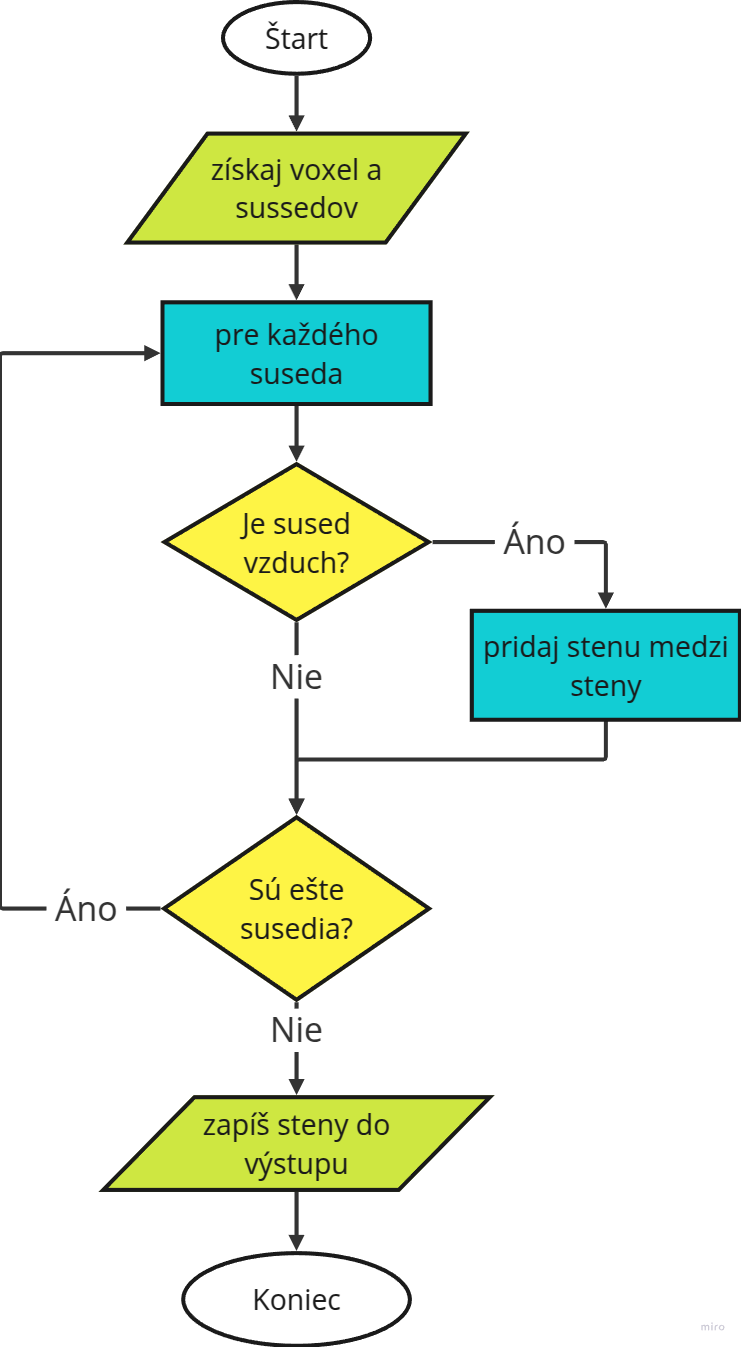
\includegraphics[height=10cm]{res/diagram_generovanie_voxelov.png}
	\caption{Znázornenie algoritmu generujúceho steny (4 vrcholy) okolo priradeného voxelu.}
	\label{obr:diagram algoritmu generujuceho vertexy}
\end{figure}

\newpage
\subsubsection{Vykresľovanie vygenerovaných dát}

Keď sú dáta vygenerované, nie je zložité ich vykresliť pomocou jednoduchého
programu pozostávajúceho z dvoch častí:

\begin{itemize}
	\item \textbf{vertex shader}, počíta, otáča a posúva body pomocou dát kamery,
	      premieta 3D body na 2D obrazovku,
	\item \textbf{fragment shader}, vyfarbuje trojuholníky tvorené vrcholmi.
\end{itemize}


\section{Výsledky práce a diskusia}

Vytvorená aplikácia Botanica demonštruje možnosť simulácie rastu rastlín
v trojrozmernom prostredí pomocou celulárnych automatov a genetického kódu.
Implementácia zahŕňa: generovanie terénu pomocou Perlinovho šumu, ktorý vytvára
realisticky vyzerajúce prostredie s variabilnou výškou a rozložením živín;
dynamické rastliny, ktoré reagujú na podmienky prostredia a menia svoj rast
na základe genetického kódu a dostupnosti živín; algoritmus rastu, ktorý
zabezpečuje prirodzenú redistribúciu živín, fotosyntézu a rozmnožovanie;
grafickú reprezentáciu založenú na voxelovom engine s renderovaním cez OpenGL,
čo umožňuje vizuálne sledovanie simulovaných procesov. Aplikácia splnila
stanovené ciele. Simulované rastliny vykazujú rôzne formy rastu na základe
ich genetického kódu a podmienok prostredia.

\begin{figure}[ht]
	\centering
	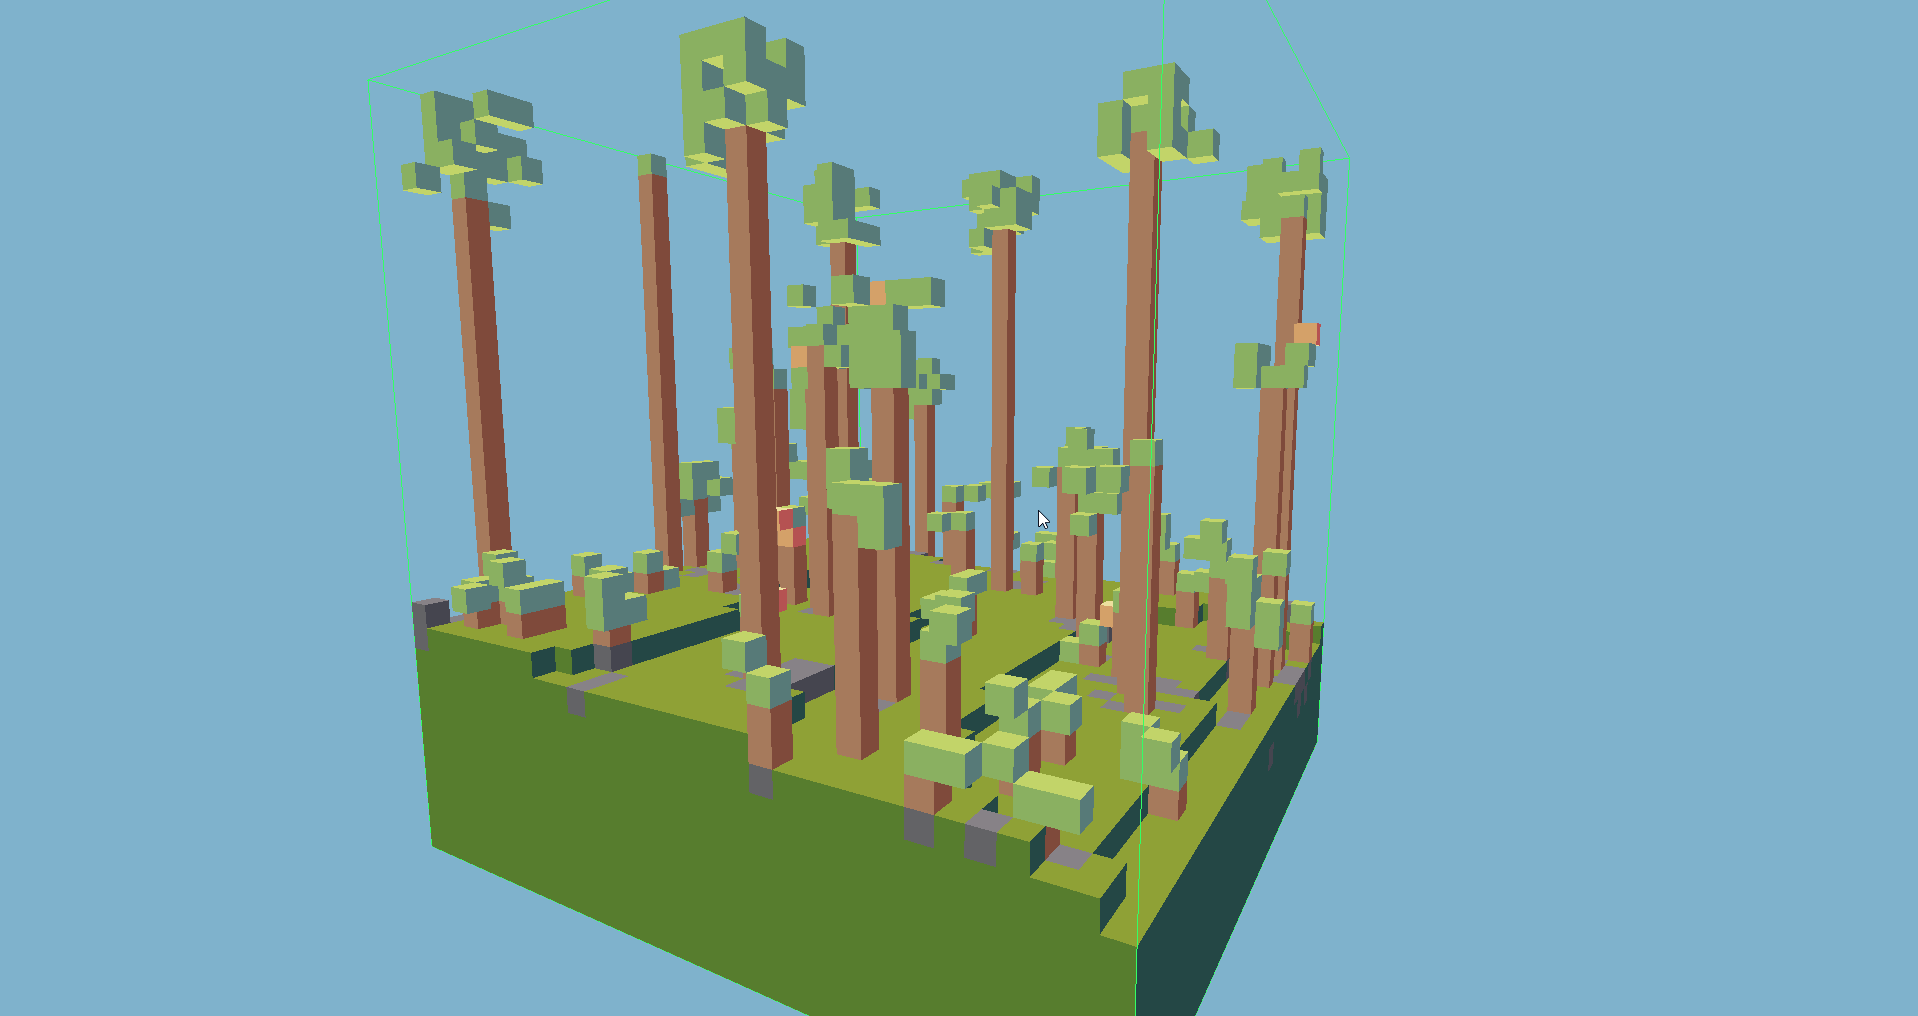
\includegraphics[width=0.7\textwidth]{res/screenshot.png}
	\caption{Snímka simulácie.}
\end{figure}

Preukázali sme, že celulárne
automaty s genetickým mechanizmom sú vhodné na modelovanie dynamického rastu
rastlín. Výsledky ukazujú, že použitie celulárnych automatov na simuláciu
rastlín poskytuje flexibilný a efektívny model. Rastliny sa dokážu adaptovať
na prostredie a meniť svoj rast podľa dostupnosti živín, čo pridáva prvok
prirodzenej selekcie.

Medzi silné stránky riešenia patrí modularita a
flexibilita - model možno rozšíriť o nové pravidlá rastu alebo iné prvky
simulácie (napr. vplyv podnebia); efektívne využitie zdrojov - využitie OpenGL
pre renderovanie ušetrilo CPU čas, čo umožnilo detailnejšiu simuláciu;
pozorovanie evolučných zmien - rastliny sa menia generáciami vďaka mutáciám
v genetickom kóde, čo demonštruje potenciál modelovania evolúcie.

Medzi slabiny riešenia a možnosti zlepšenia patrí obmedzená komplexnosť
genetiky - aj keď genetický kód ovplyvňuje rast, model zatiaľ neobsahuje
komplexnejšie mechanizmy; statické podmienky prostredia - simulácia zatiaľ
nezahŕňa dynamické faktory ako meniace sa počasie alebo sezónne zmeny.

Napriek týmto obmedzeniam je Botanica silným východiskovým bodom pre ďalší
výskum v oblasti simulácie rastlín a evolučných procesov v digitálnych
ekosystémoch.

\section{Závery práce}

Táto práca sa zamerala na návrh a realizáciu simulácie rastu rastlín pomocou
bunkových automatov. Tento prístup sa ukázal ako efektívny pri modelovaní
dynamických procesov rastu, avšak počas vývoja sa vyskytlo viacero výziev,
ktoré ovplyvnili priebeh implementácie. Medzi najvýznamnejšie patrila
implementácia algoritmu do jazyka C++, keďže pre 2 členov týmu tento jazyk
bol pred začatím práce neznámi a mali celkovo limitované poznatky
z programovania. Niektoré technické aspekty, najmä správa pamäte a efektívne
vykresľovanie voxelového priestoru, si vyžadovali dodatočné úpravy
a optimalizáciu. Tieto poznatky priniesli cenné skúsenosti, ktoré môžu byť
využité v budúcnosti.

Jedným z hlavných zistení bolo, že aj jednoduché pravidlá bunkových automatov
môžu viesť k vzniku komplexných a realistických štruktúr. Tento výsledok
potvrdzuje vhodnosť zvoleného prístupu a naznačuje možnosti ďalšieho rozšírenia
modelu o sofistikovanejšie faktory, ako je implementácia zvierat do systému,
zrážky alebo ročné obdobia.

Napriek uvedeným výzvam sa podarilo vytvoriť funkčný model, ktorý ponúka rôzne
možnosti konfigurácie a experimentovania s parametrami rastu. Táto práca môže
slúžiť ako základ pre ďalší výskum a aplikácie v oblastiach, hlavne v simuláciách
rastlinných systémov v počítačových hrách.


\section{Zhrnutie}

Cieľom tejto práce je navrhnutie možnej alternatívy, alebo rozšírenia,
ku procedurálnemu generovaniu rastlín, ktorá umožňuje rastlinám reagovať na
prostredie v~ktorom sa nachádzajú, čím sa spestrí svet pre hráča. Táto práca
predstaví ako demonštráciu Aplikáciu, ktorá pre oživenie procedurálne
generovaného sveta využíva algoritmus simulujúci základné procesy rastlín.
Aplikácia sa skladá z troch častí: generovanie malej časti trojrozmerného
voxelového sveta pomocou perlinovho šumu, algoritmus na simuláciu rastlín
inšpirovaným celulárnymi automatmi a~renderovanie tejto časti sveta s
využitím grafického API OpenGL.


\nocite{*} % print the whole bibliography
\renewcommand{\refname}{Zoznam použitej literatúry}
\bibliography{soc}
\addcontentsline{toc}{section}{Zoznam použitej literatúry}

\end{document}
